\chapter{Objetivos do trabalho}
\label{chapterObjetivos}
\section{Transistores \textit{wide bandgap}: GaN}
Segundo a \textit{World Semiconductor Trade Statistics}, cada pessoa no planeta comprou uma média de 111 chips ou circuitos integrados (ICs) em 2016. O uso desses dispositivos semicondutores está crescendo cinco vezes a taxa de crescimento da população humana \cite{Sameer}. Natural que haja uma busca por dispositivos que possibilitem maior densidade de transistores, bem como menor dissipação de energia na forma de calor. Transistores de Nitreto de Gálio e Carbeto de Silício vem se mostrando como alternativa ao cenário atual, com Silício. No caso do Nitreto de Galio, são bons chaveadores em alta frequência além baixa resistência quando ligados \cite{lidow_rooij_strydom_reusch_glaser_2020}. 
\par Assim, o emprego de transistores GaN apresenta grande vantagem quando inserido em aplicações sensíveis à eficiencia energética, especialmente como dispositivos portáteis ou à bateria, além de dar mais flexibilidade ao projeto, uma vez que ao chavearem em mais alta frequência, elementos magnéticos menores podem ser usados nos projetos de fontes chaveadas, por exemplo.  
\par Neste trabalho, transistores do tipo GaN serão empregados em um sistema solar fotovoltaico de pequeno porte para alimentação de uma bateria Li-Ion(18650) como na figura \ref{FigDiagBlocoSistema}.
\par Os capitulos \ref{chapterObjetivos} e \ref{chapterRevisao} contextualizam e definem modelos matemáticos necessários para aplicação do transistor tipo GaN em fontes chaveadas, nos capítulos \ref{chapterMetodologia} será apresentado a simulação computacional dos modelos descritos nos capitulos anteriores. Os resultados parciais dos blocos já simulados e analises já encaminhadas se encontam no capitulo \ref{chapterResultados}.

\begin{figure}[H]
\caption{Diagrama de blocos} 
\begin{center}
\begin{circuitikz}
%Coluna,Linha
%(0,0) botton left

\draw %painel solar
    (0,0)   to [short,i=] (3,0)
    (3,0)   to [short] (3,3)
    (3,3)   to [short] (0,3)
    (0,3)   to [short] (0,0)
    (1.5,1.5) node[]{Painel Fotovolt.};

\draw %MPPT
    (3.5,-1)   to [short,i=] (5.5,-1)
    (5.5,-1)   to [short,i=] (5.5,-2)
    (5.5,-2)   to [short,i=] (3.5,-2)
    (3.5,-2)   to [short,i=] (3.5,-1)
    (4.5,-1.5) node[]{MPPT};

\draw %buck
    (6,0)   to [short,i=] (9,0)
    (9,0)   to [short] (9,3)
    (9,3)   to [short] (6,3)
    (6,3)   to [short] (6,0)
    (7.5,1.5) node[]{Buck};

\draw %Controle
    (6,-1)   to [short,i=] (9,-1)
    (9,-1)   to [short,i=] (9,-2)
    (9,-2)   to [short,i=] (6,-2)
    (6,-2)   to [short,i=] (6,-1)
    (7.5,-1.5) node[]{Controle};

\draw %bateria   
    (12,2.5)   to [battery,i=] (12,-1)
    node[ground]{};

\draw %Connections    
    (3,2.5)   to [ammeter] (6,2.5)
    (3,0.5)   to [short] (6,0.5)
    (3.5,0.5) to [voltmeter,*-*] (3.5,2.5)
    
    (11,-1) to [voltmeter,-*] (11,2.5)
    (11,-1) node[ground]{}
    (9,2.5)   to [ammeter] (11,2.5)
    (11,2.5)   to [short] (12,2.5)
    
    (4.5,2.1) to [short] (4.5,-1)
    (4.1,1.5) to [short] (4.1,-1)
    (3.9,1.5)   to [short] (4.1,1.5)
    
    (5.5,-1.5)   to [short] (6,-1.5)
    (7.5,-1)   to [short] (7.5,0)
    ;
\end{circuitikz}
\end{center}
\label{FigDiagBlocoSistema}
\end{figure}
%\begin{figure}[H]
%\caption{Diagrama de bloco}
% \centering % para centralizarmos a figura
%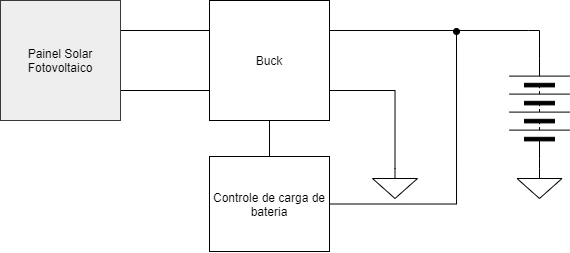
\includegraphics[width=6cm]{figuras/DiagramaBlocos.png} 
%\label{FigDiagBlocoSistema}
%\end{figure}


\section{Paineis solares fotovoltáicos}
%REESCREVER - CÓPIA DO ARTIGO DO BRANDAO/VILALLVA - trocar o título talvez
%\par A escolha do sistema utilizado passa pela necessidade de acesso a energia em comunidades remotas e carentes, que em grande parte das vezes não conseguem acesso nem ao mais basico acesso à energia elétrica. Isso limita a rotina, o convívio social e ainda expõe esses brasileiros a diversos riscos, como ataques de animais. Além disso, o uso de lamparinas para suprir a ausência de eletricidade afeta a saúde da população e pode causar incêndios nas casas.
%\par Diante deste cenário, um sistema de energia solar de pequeno porte, que carregue uma bateria é vital para manter iluminação e para carregar pequenos dispositivos, garantindo assim aumento na qualidade de vida como um todo. 
%\par A associação Pisco de Luz \cite{pisco} faz um trabalho importante para alterar esta realidade. 
%\par O sistema solar fotovoltaico é composto por um painel solar fotovoltaico, conversores chaveados e, podem ou não ser conectados à rede elétrica.\\
%...
%Esperar livro do Marcelo Vilalva.
%\par Majoritariamente, a fonte de energia do nosso planeta é solar, seja na forma de luz ou calor. \cite{Villalva}.
%\par As fontes de energias renováveis vêm desempenhando um importante papel no cenário mundial, principalmente devido à crescente preocupação com
%o meio ambiente – efeito estufa e aquecimento global– e ao contínuo aumento da demanda energética.Neste contexto, os sistemas de geração distribuída
%despertam grande interesse, pois podem utilizar diversos tipos de fontes primárias de energia, podem ser instalados próximos às cargas e atenuam as necessidades imediatas dos governos em realizar investimentos onerosos na matriz energética (XuWei,2009, Pomílio, 2011).
%\par Um conjunto controlado de sistemas de geração distribuída e cargas locais pode ser denominado microrrede. Uma microrrede pode ser entendida como um pequeno sistema de energia elétrica controlável que pode, entre outras coisas, auxiliar as concessionárias no processo de despacho de energia,redução das perdas no processo de transmissão e correção de afundamentos de tensão. Pode ainda ser desconectado automaticamente do sistema de distribuição em casos de faltas elétricas ou intencionalmente, de acordo com a vontade do usuário (Lasseter, 2007 e Kroposki, 2008). 
%\par A energia fotovoltaica se destaca das outras fontes renováveis e limpas principalmente pelo fato de poder ser instalada rapidamente em comércios e
%residências, além de ser silenciosa e inesgotável (Barker, 2005). As principais desvantagens dos sistemas fotovoltaicos são a baixa eficiência dos módulos comerciais de silício cristalino, que atualmente está em torno de 15\% e, o elevado custo de instalação, devido aos módulos e aos conversores eletrônicos.
%\par Os sistemas de geração distribuída podem operar como sistemas autônomos e/ou sistemas interligados à rede elétrica. O primeiro tipo é fundamental para o processo de inclusão social, fornecendo energia elétrica às propriedades que não têm acesso ao sistema de distribuição. O segundo tipo, que pode ser usado em zonas urbanas e densamente povoadas, é mais interessante por sua contribuição ao sistema elétrico nacional, pois pode aliviar os picos de demanda e as linhas de transmissão e de distribuição, que já operam em sua capacidade máxima \cite{BrandaoVilallalva}.